\documentclass[10pt, twoside]{article}
\usepackage{main}

% Aquí empieza el documento{{{
\begin{document}

%\maketitle
\thispagestyle{fancy}

% Carátula {{{
\begin{center}
	$1^{\text{ER}}$ LABORATORIO DE FÍSICA $2$
	%Informe del Laboratorio N° 1
\end{center}

\noindent
\begin{tikzpicture}
	\tikzmath
	{
		coordinate \xMa;
		\xMa = (\textwidth-1.6pt,0);
	}
	\draw [ultra thick](0,0) rectangle ++(\xMax*0.8,-5)
		++(0.25,0)
		rectangle (\xMax,0);

	\draw(2,-.5) node {Título del laboratorio};
	\draw({(\xMax*0.8+\xMax)/2},-.5) node {NOTA};
\end{tikzpicture}

\bigskip
\bigskip
\bigskip
\noindent
%\begin{tikzpicture}
	%\tikzmath
	%{
		%coordinate \xMa;
		%\xMa = (\textwidth-0.4pt,0);
	%}
	%\foreach \x in {0, ..., 5}
	%{
		%\draw ({\x*\xMax/6},0) rectangle ++(\xMax/6,0.75);
	%}
	%\draw (0.62,0.4) node {\textbf{Fecha}}
		%++(\xMax/3,0) node {\textbf{Hora}}
		%++(\xMax/3,0)++(0.4,0) node {\textbf{Ambiente}}
		%;
%\end{tikzpicture}

\bigskip
\bigskip
\noindent
\begin{tikzpicture}
	\tikzmath
	{
		coordinate \xMa;
		\xMa = (\textwidth-0.4pt,0);
	}
	\foreach \y in {0,1}
	{
		\draw (0,\y) rectangle +(\xMax*0.5,-1)
			++(\xMax*0.5,0) rectangle ++(\xMax*0.25,-1)
			+(0,1) rectangle (\xMax,\y-1);
	}
	\draw (\xMax*0.25,0.7) node {\textbf{Integrantes}}
		++(\xMax*0.38,0) node {\textbf{Código}}
		++(\xMax*0.25,0) node {\textbf{Participación}}
		++(0,-0.4) node {\textbf{(\%)}}
		;
	\draw (\xMax*0.25,0.7-1) node {Alberto Oporto Ames}
		++(\xMax*0.38,0) node {$201810518$}
		++(\xMax*0.25,0) node {100\%}
		;
\end{tikzpicture}
% }}}

\newpage

\section{EXPERIENCIA A:Observación de superficies equipotenciales y líneas de
campo eléctrico}%

\subsection{OBJETIVOS}%

Escribir en una tabla las coordenadas de los puntos en los que
el voltaje es el mismo.

\subsection{PROCEDIMIENTO Y ANÁLISIS}%

\begin{table}[H]
	\centering
	\caption{Coordenadas}
	\label{tab:coordenadas}
	\begin{tabular}{c|c||c|c||c|c||c|c}
		\multicolumn{2}{c||}{$2V$}
		&\multicolumn{2}{c||}{$3V$}
		&\multicolumn{2}{c||}{$4V$}
		&\multicolumn{2}{c}{$4.5V$}\\
		\hline
		\hline
		x & y & x & y & x & y & x & y\\
		\hline
		$-10U$ & $1U$ & $-6.5U$ & $-5U$ & $4U$ & $7U$ & $10U$ & $9U$\\
		\hline
		$-12U$ & $-1U$ & $-5U$ & $-1U$ & $4U$ & $5U$ & $13U$ & $12U$\\
		\hline
		$-14U$ & $-2U$ & $-4U$ & $1U$ & $3U$ & $3U$ & $5U$ & $-10U$\\
		\hline
		$-16U$ & $-3.5U$ & $-3U$ & $5U$ & $2U$ & $0U$ & $4U$ & $-5U$\\
		\hline
		$-18U$ & $-4U$ & $-2U$ & $8U$ & $-2U$ & $-2U$ & $4U$ & $-2U$\\
		\hline
		$-8U$ & $4U$ & $-2U$ & $12U$ & $2U$ & $-4U$ & $4U$ & $0U$\\
		\hline
		$-7U$ & $7U$ & $-6U$ & $-10U$ & $1.5U$ & $-5U$ & $5U$ & $3U$\\
		\hline
		$-7.5U$ & $10U$ & $-7U$ & $-7U$ & $2U$ & $-9U$ & $7U$ & $6U$\\
		\hline
	\end{tabular}
\end{table}

\begin{figure}[H]
	\centering
	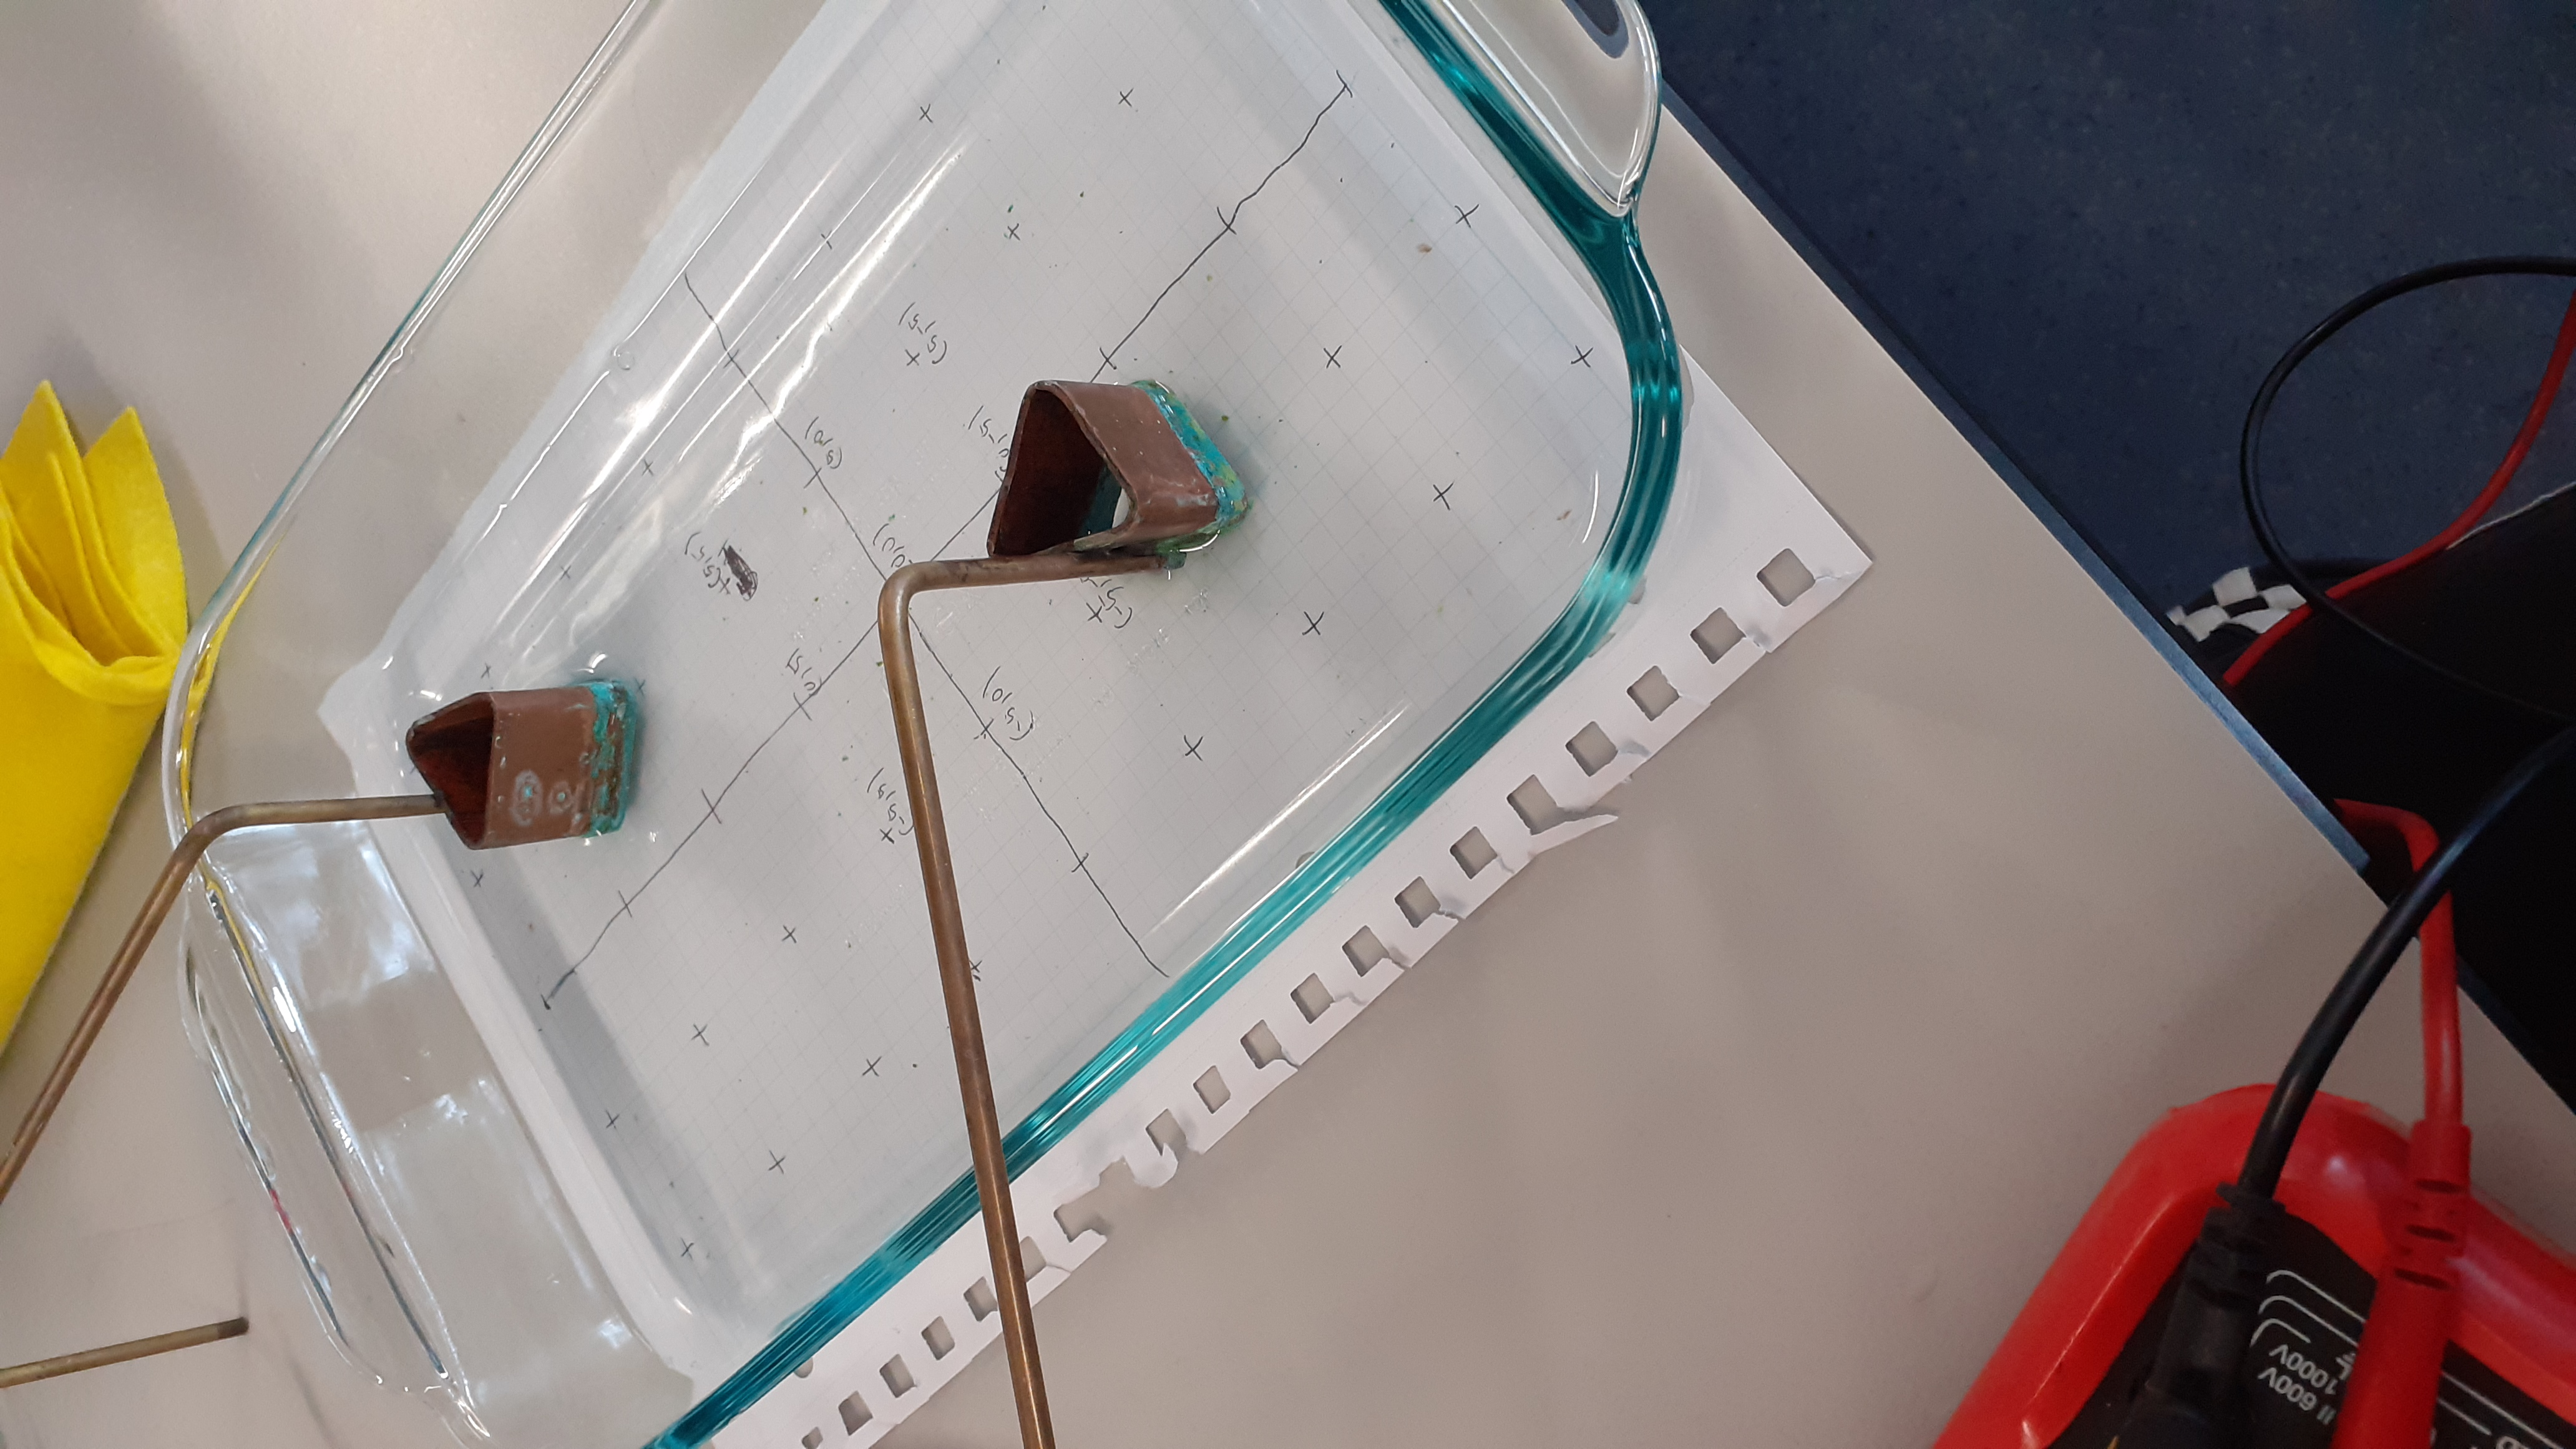
\includegraphics[width=0.8\linewidth, angle=-90]{20190917_152938.jpg}
	\caption{Electrodos en una bandeja}%
	\label{fig:bandeja}
\end{figure}

\subsection{COMENTARIOS Y OBSERVACIONES}%

Tuve que tomar datos dos veces,
dibujar mis ejes de coordenadas 3 veces
y por unos días pensé que había perdido mi hoja con los datos.

\subsection{CUESTIONARIO}%

\begin{enumerate}[label=\roman*]
	\item Dibujar las líneas de campo y las líneas equipotenciales en la hoja
		cuadriculada, no olvidar de dibujar el contorno y la posición de los
		electrodos usados.
	\item Aproximar la carga de los electrodos al centro de los mismos,
		mostrar el cálculo para obtener la carga total del electrodo.
	\item Escoger $3$ puntos que pertenecen a las líneas equipotenciales
		dibujadas y aproximar el valor de la intensidad de campo
		eléctrico (mostrar los cálculos) y también mostrar la dirección
		aproximada del vector intensidad de campo eléctrico.
\end{enumerate}

\subsection{CONCLUSIONES}%


\section{EXPERIENCIA B:Carga y descarga de un condensador}%

\subsection{OBJETIVOS}%

Grabar con un celular un multímetro y gastar casi toda mi
memoria libre.

\subsection{PROCEDIMIENTO Y ANÁLISIS}%

\begin{figure}[H]
	\centering
	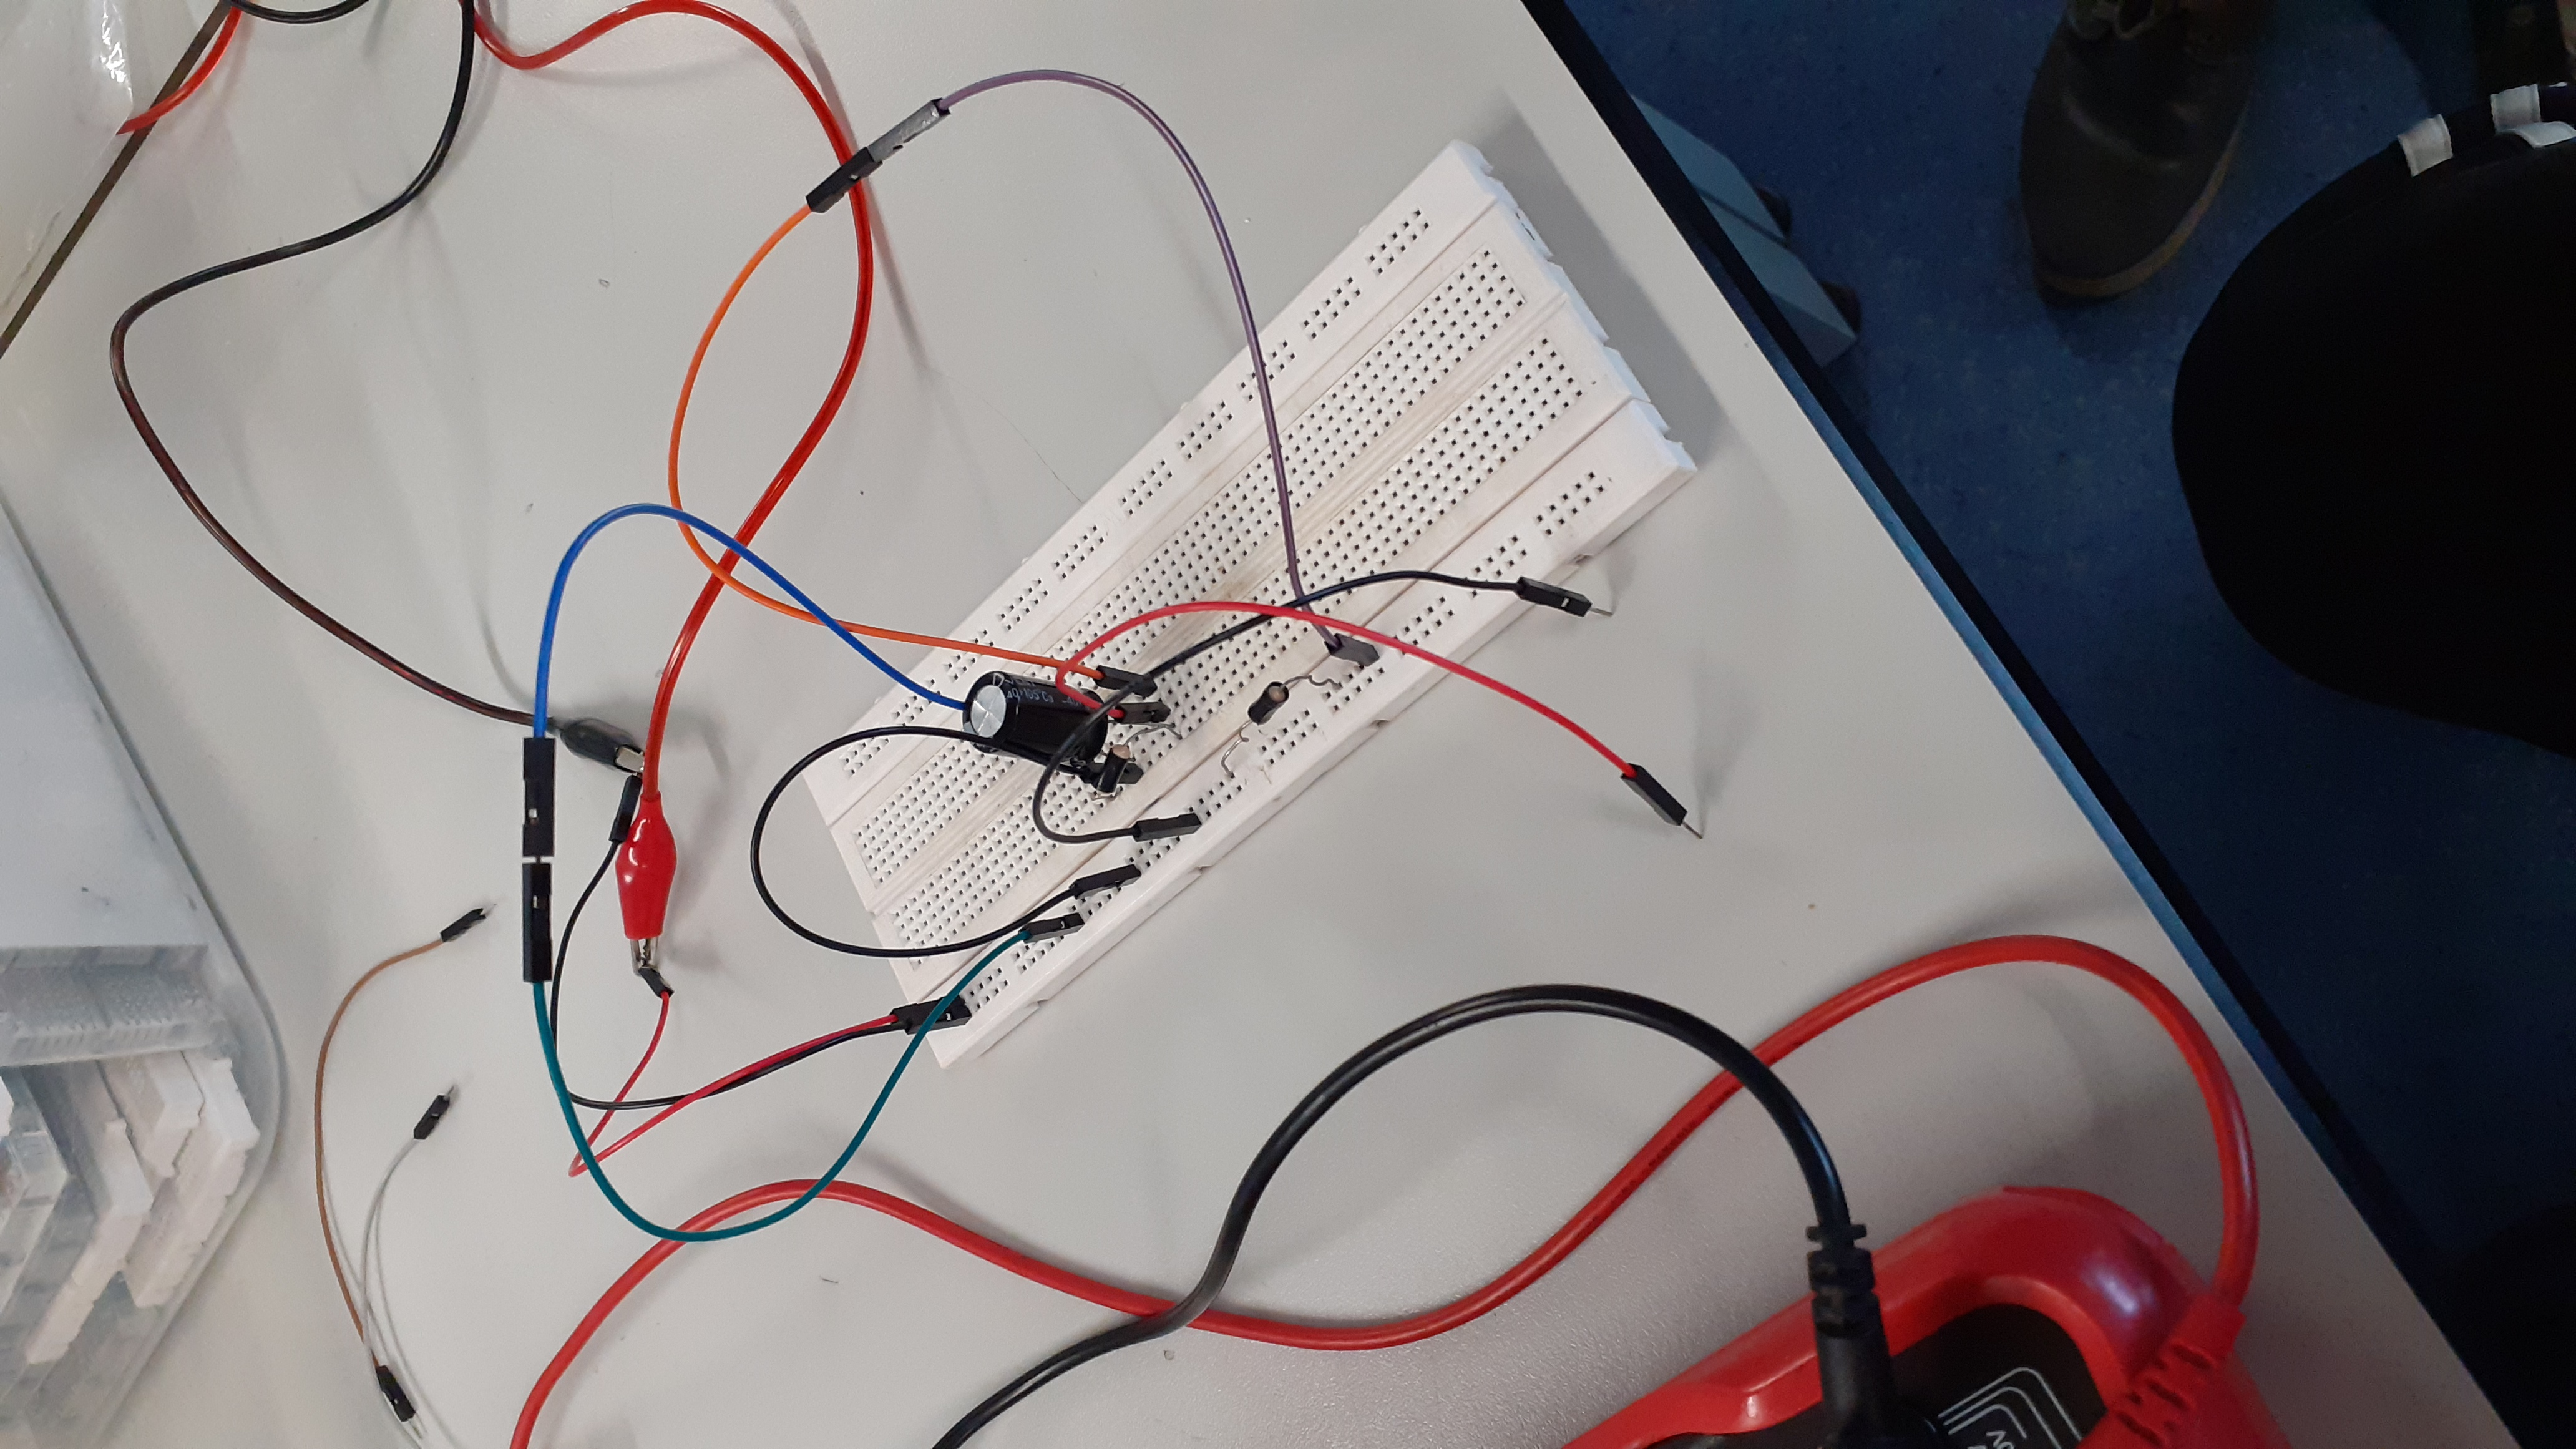
\includegraphics[width=0.8\linewidth, angle=-90]{20190917_163108.jpg}
	\caption{Un Breadboard}%
	\label{fig:bread}
\end{figure}

\subsection{COMENTARIOS Y OBSERVACIONES}%

No había el medidor logger pro de la guía,
así que tuve que medir el voltaje con un multímetro y mi celular.

\subsection{CUESTIONARIO}%
\begin{enumerate}[label=\roman*]
	\item Mostrar y resolver la ecuación diferencial obtenida al aplicar la
		leyes de Kirchhoff en un circuito $RC$.
		Mostrar la ecuación de voltaje respecto a tiempo que se debería
		obtener de manera teórica.
	\item Comparar las funciones de carga y descarga observadas con las
		funciones obtenidas en el ítem anterior.
		Usar \textbf{PGFPLOTS} para realizar la comparación de las funciones.
	\item Aproximar los valores de la resistencia $R_1$ y $R_2$ utilizando
		las gráficas obtenidas de carga y descarga.
		Utilizar todos los puntos y obtener valores promedio de resistencias.
\end{enumerate}

\subsection{CONCLUSIONES}%

\section{EXPERIENCIA C:Cuantificación del campo magnético}%

\subsection{OBJETIVOS}%

Poner un palo dentro de unos aros y copiar, del logger pro, la magnitud promedio
del campo magnético.

\subsection{PROCEDIMIENTO Y ANÁLISIS}%

\subsection{COMENTARIOS Y OBSERVACIONES}%

Al inicio conecté la bobina con unos cocodrilos.
La intensidad seguía siendo $0A$ y no había campo magnético.

Tenía que usar esos conectores que parecen dispensadores de gasolina.

\subsection{CUESTIONARIO}%
\begin{enumerate}[label=\roman*]
	\item Utilizando las mediciones de campo magnético para una bobina,
		estimar el valor de su número de vueltas $N$.
	\item Utilizando el valor de $N$ hallado en el paso anterior,
		determina el valor teórico en el punto en el que se realizó la medición
		utilizando dos bobinas.
		Compara esto con el valor medido,
		y halla el porcentaje de error respecto al valor teórico.
\end{enumerate}

\subsection{CONCLUSIONES}%

\end{document}
%}}}
